\documentclass[a4paper]{article}
\usepackage[english]{babel}
\usepackage[utf8]{inputenc}
\usepackage{amsmath}
\usepackage{graphicx}
\usepackage{tikz}
\usepackage{dot2texi}
\usepackage{pgfplots}
\usepackage{algorithm}
 \usepackage{verbatim}
\usepackage{graphicx}
\usepackage{color}
\usepackage{epsfig}
\usepackage{multirow}
\usepackage{amsfonts}
\usepackage{hyperref}
\usepackage{wrapfig}
\usepackage{algpseudocode}
\usepackage[colorinlistoftodos]{todonotes}
\usepackage{geometry}
 \geometry{
 a4paper,
 total={210mm,297mm},
 left=20mm,
 right=20mm,
 top=10mm,
 bottom=15mm,
 }



\title{Modeling Blockchain based Lottery protocol in Tamarin}
\author{Parag Bansal}
\date{June 2017}
\begin{document}
\maketitle
\section{Bitcoin}

Bitcoin is digital currency protocol introduced in 2008. It is a decentralized protocol which lacks any central authority and the list of all the transactions are kept in publicly available ledger called blockchain. Transfer of money from one party to another party is done by requesting a transaction, digitally signed by the private key. Miners verify such request and club many such request to form a block, and blocks are then linked into the blockchain.\\

\subsection{Currency Flow}

\begin{wrapfigure}{r}{0.5\textwidth}
  \begin{center}
  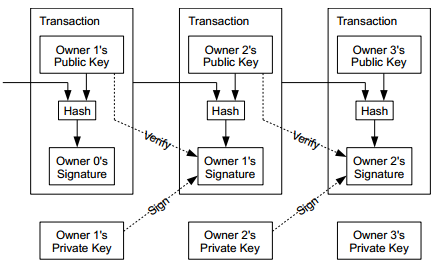
\includegraphics[width=0.48\textwidth]{bitcoin.png}
  \end{center}
  \caption{Transaction structure}
\end{wrapfigure}
A coin owner transfers coins by digitally signing a hash digest of the previous transaction(unspent) and the public key of next owner. New coins are generated due to mining process, miner receives a block reward on solving a block puzzle.\\ Note that syntax of bitcoin allows for more advanced transactions than simply transferring money. Each bitcoin transaction has an output script(A boolean function) associated with it, which must be evaluated to true for redeeming that transaction. In simple case, the boolean function requires signature to be evaluated to true, but you can specify advanced conditions. Every transactions take few(more than or equal to one) previously posted transactions which are not redeemed as input, along with the input(signature simply) to satisfy the boolean function of each input transaction.
\subsection{Double Spending}
The most important problem with any digital currency is the problem of double spending since coins are just bit string, owner can spend it multiple times. This can be avoided if everyone has access to a trusted ledger which keeps track of transactions but that would defeat the purpose, as we are looking for decentralized protocol. Bitcoin tackles this problem by using blockchain. Miners pick unconfirmed transactions and put them in a block after solving a moderately difficult block puzzle. Note that, at time of creating a block miner verify, whether the input transactions have not been redeemed previously and all the boolean functions of this transaction evaluates to true.\\
Since many miners are simultaneously working on solving block, it might be the case that multiple miners end up solving a block simultaneously. In such cases blockchain forks to form a tree like structure. Longest length path in this tree is always the accepted blockchain, and miners try to append the block to longest path.\\
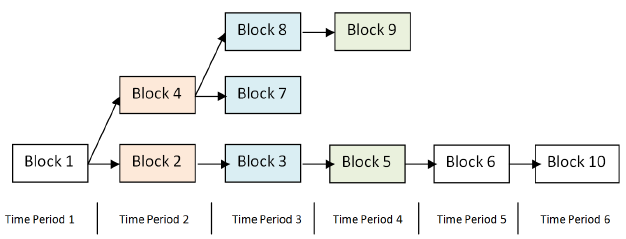
\includegraphics[width =0.5\textwidth]{bitcoin2.png}
\\If an adversary has to do a double spending attacks then it has to invalidate all the blocks that come after the block which contains the transaction, i.e. miner has to create a longer blockchain and mine a lot of blocks. Note that, a miner is in race with rest of the network so to mine a large number of blocks faster than other, it should have access to more 51\% of world's computing power. 
\begin{center}
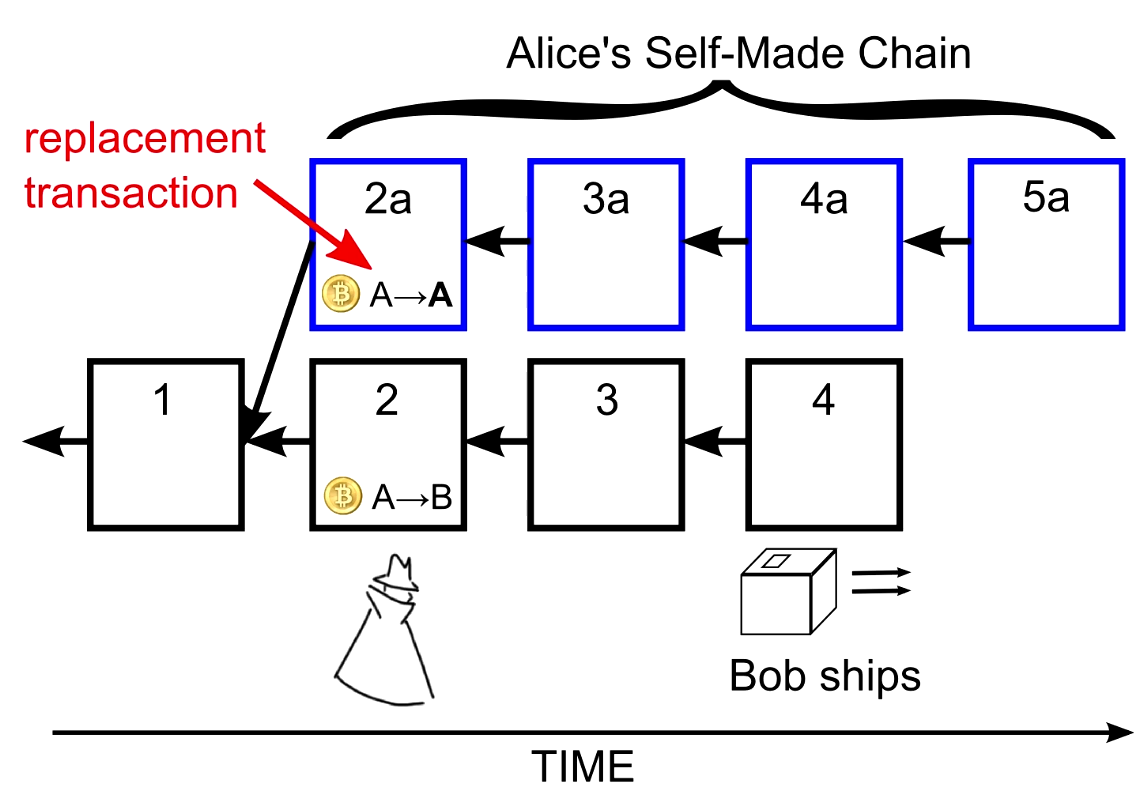
\includegraphics[width = 0.5\textwidth]{bitcoin3.png}
\end{center}
\section{Lottery Protocol}
Secure multiparty computation is field with goal of creating methods for parties to jointly compute a function on their private inputs. Its application include gambling and lottery. It is not very difficult to design such protocols in presence trust-worthy central authority, but decentralized versions of such protocols which does not require such an authority have suffered from lot of security issues including fairness and liveness.\\

Bitcoin provides an interesting way for multi-party computations, as it's a decentralized digital currency and blockchain technology of bitcoin can be utilized for modeling central authority type of entity. Note that in addition to simple transactions bitcoin also provides a way to write timed commitments and some other ways to write complex scripts for redeeming the money.\\ 
Any bitcoin transaction involves, a previously posted redeemable transaction, an input script which provides a signature to redeem previously posted and transaction, an output script specifying how this transaction can be redeemed in future and in certain transactions a time-stamp field specifying when can this transaction be redeemed.\\
\begin{center}
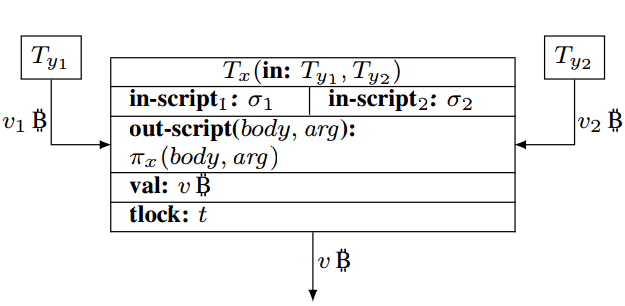
\includegraphics[width =0.5\textwidth]{bitcoin5.png}
\end{center}
\subsection{Bitcoin based timed-commitments}
A commitment scheme is generally executed between two parties: namely a committer C and recipient. The committer starts the protocol with some secret value x, and with the agreement that this value will be known to participants after the opening phase is executed. Now, a dishonest committer can change his mind and might reveal a value different from x. Trivially, there is no way to force committer to reveal the same value. We can utilize blockchain technology to force committer reveal the same value using timed commitments. A committer chooses a value x, and posts a transaction whose signature requires value x to revealed, while simultaneously posting a another timed transaction which utilizes the same un-redeemed transaction in the name of recipient. This ensures that committer will have to reveal the secret x before time t, otherwise recipient will be able to redeem the transaction.\\
\begin{center}
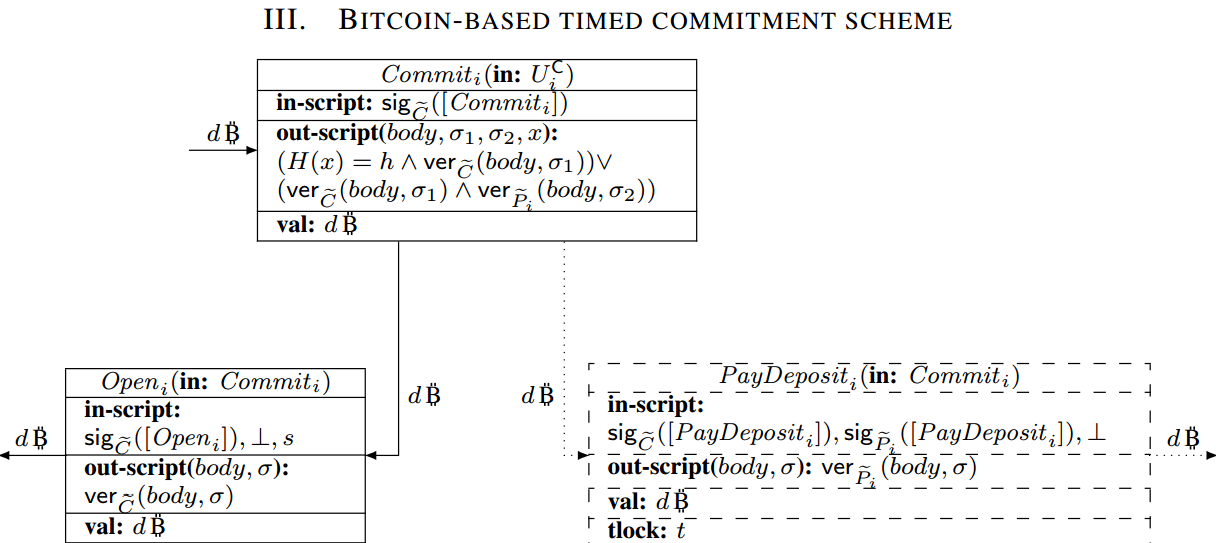
\includegraphics[width = 0.5\textwidth]{bitcoin6.png}
\end{center}
\subsection{Two party Lottery protocol}
A lottery protocol essentially means that each party will choose a random number and a winner will be decided by evaluating a function on all the numbers. In case of two parties, one such function could be sum of numbers modulo two. If it's odd then 1st party wins otherwise second.
\subsection{Protocol Description}
Lets say Alice and Bob are two participants of protocol with their pairs of keys $(\widetilde{A},\widetilde{B})$. Both Alice and Bob start by choosing their secret string $s_A$ and $s_B$, respectively and exchange the hashes $H(s_a)$ and $H(s_b)$. Alice sends the following transaction $PutMoney^A$ to ledger. Bob also sends a transaction $PutMoney^B$ defined symmetrically.\\
\begin{center}
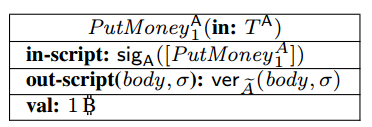
\includegraphics[width = 0.5\textwidth]{bitcoin7.png}.\\
\end{center}
These PutMoney transaction are then used to create a compute transaction whose output script is such that it can be redeemed only by the winner of the lottery, and the value of the transaction is sum  of these PutMoney transactions.\\
\begin{center}
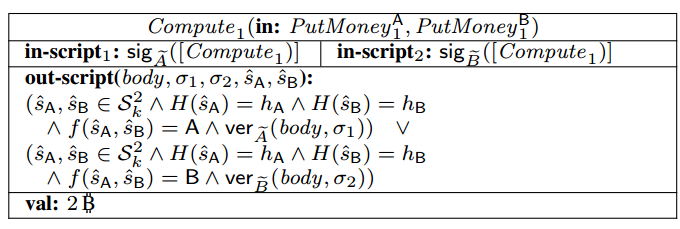
\includegraphics[width = 0.5\textwidth]{bitcoin8.png}\\
\end{center}
Note that, output script of compute is alternative of two condition. if $f(s_A, s_B) = A$ then it can be redeemed using the signature of A, otherwise it can be redeemed using the signature of B. This ensures that any party can not unfairly redeem the transaction.\\ Clearly, once the compute transaction appears on ledger, parties can not change their mind and redeem their PutMoney transaction since it had been already been redeemed by compute transaction. Now, Final step is that Alice and Bob just broadcast their secrets, $s_A$ and $s_B$ respectively, and then the winner can redeem the compute transaction using ClaimMoney as follows.\\

\begin{center}
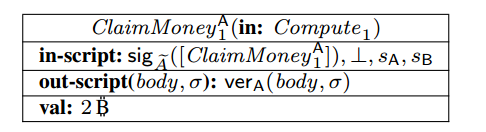
\includegraphics[width = 0.5\textwidth]{bitcoin9.png}\\
\end{center}
This protocol is obviously correct. Unfortunately, it suffers from the following problem, there is no guarantee that the parties always send $s_A$ and $s_B$. If any party refuses to reveal his secret after the commit phase then both parties money is lost. This is exactly why we need timed commitments to solve this problem.
\section{Tamarin Model}
\subsection{Tamarin-Prover}
Tamarin prover is powerful tool for symbolic modeling and analysis of security protocols. It takes as input a protocol model, specifying the actions taken by agents running the
protocol in different roles(e.g. initiator, responder), a specification of the adversary, and a specification of the protocol’s desired properties. We write the desired security properties of protocol in form of lemmas, while action of agents are specified as rules using multiset rewrite rules. \\
A rewrite rule in Tamarin has a name and three parts, each of which is a sequence of facts: one for
the rule’s left-hand side, one labelling the transition (which we call 'action facts'), and one for the rule’s right-hand side.\\
Initial state of the transition system is empty multiset. The rules define how the system can make a transition to a new state. A rule can be applied to a state if it can be instantiated such that its left hand side is contained in the current state. In this case, the left-hand side facts are removed from the state, and replaced by the instantiated right hand side.\\

\subsection{Model}
To find the security flaws in this protocol, we will try to model this blockchain based protocol in tamarin-prover.



\end{document}
